\section{\label{sec:theory}Theoretical Background}

\subsection{The Electrokinetic Equations}

In the following, we will derive the equations modeling the time evolution of the concentrations of dissolved species as well as the solvent in the standard electrokinetic model. We do so, neglecting the salt ions' contribution to the overall mass density, which allows us to treat the dynamics of the ions and the fluid separately~\cite{degraaf14a}. The solvent fluid will be modeled using the Navier-Stokes equations while we use a set of diffusion-migration-advection equations for the ionic species.

\subsubsection{\label{sub:species}Ionic Species}

The description starts with the ionic species' concentrations $c_{k}(\vec{r}, t)$ (number density) and the associated flux densities $\vec{j}_{k}(\vec{r}, t)$, for which mass conservation holds
%
\begin{equation}
\label{eq:model_continuity}
\partial_{t} c_{k} = -\nabla \cdot\vec{j}_{k} . 
\end{equation}
%
Here $\vec{r}$ denotes the spatial coordinate and $t$ the time, while $k$ enumerates the ionic species. The fluxes are caused by diffusion (due to density variations and external forces) and advection.

The advective contribution to the flux is given by
%
\begin{equation}
\label{eq:adv_flux}
\vec{j}_{k}^{\mathrm{adv.}} = c_{k} \vec{u} ,
\end{equation}
%
where $\vec{u}(\vec{r}, t)$ denotes the fluid velocity (advective velocity). Equation~\eqref{eq:adv_flux} models advection as a simple co-movement of the dissolved ions with the surrounding fluid. All inertial effects of the ions are neglected.

The diffusive behavior of the ions is best described in a reference frame co-moving with the local advective velocity $\vec{u}$. We assume that the species' relative fluxes instantaneously relax to a local equilibrium. This assumption allows us to derive the diffusive fluxes from a local free-energy density, which we define as
%
\begin{equation}
\label{eq:model_free_energy}
f \big( c_{k}(\vec{r}) \big) = \sum_{k} \underbrace{\kT c_{k}(\vec{r}) \left[ \log \left\lbrace \Lambda_{k}^{3} c_{k}(\vec{r}) \right\rbrace - 1 \right] }_{\mathrm{ideal~gas~contribution}} + \underbrace{z_{k} e c_{k}(\vec{r}) \Phi(\vec{r})}_{\mathclap{\mathrm{electrostatic~contribution}}} ,
\end{equation}
%
with the $\Lambda_{k}$ the species' thermal de Broglie wavelengths, $z_{k}$ their valencies, and $\Phi(\vec{r})$ the electrostatic potential. This free-energy density consists of only an ideal-gas and an electrostatic contribution. The same assumptions form the basis of Poisson-Boltzmann (PB) theory. Hence, the limitations of this model are the same as those of PB. That means this model applies to monovalent ions at low to intermediate densities and surface charges~\cite{punkkinen08a,degraaf12a}.

The species' chemical potentials $\mu_{k}$ implied by the free-energy density read
%
\begin{equation}
\label{eq:chempot}
\mu_{k}(\vec{r}) = \delta_{c_k} f(c_{k}\big( \vec r ) \big) = \kT \log(\Lambda_{k}^{3} c_{k}(\vec{r})) + z_{k} e \Phi(\vec{r}) .
\end{equation}
%
This in turn allows us to formulate first-order approximation to the thermodynamic driving force as the gradient of the chemical potential~\eqref{eq:chempot}, which we use to define an expression for the diffusive flux
%
\begin{equation}
\begin{aligned}
\label{eq:model_jdiff}
\vec{j}_{k}^{\mathrm{diff}} &= \xi_{k} \left( -c_{k} \nabla \mu_{k} \right) = -\kT \xi_{k} \nabla c_{k} - \xi_{k} z_{k} e c_{k} \nabla\Phi \\
& = -D_{k} \nabla c_{k} - \xi_{k} z_{k} e c_{k} \nabla \Phi . 
\end{aligned}
\end{equation}
%
Here, $\xi_{k}$ and $D_{k}$ denote the mobility and the diffusion coefficient of species $k$, which are related by the Einstein-Smoluchowski relation $D_{k} / \xi_{k} = \kT$~\cite{einstein1905a,smoluchowski1906a}.

Finally, the total number density flux combining effects of diffusion and advection reads
%
\begin{equation}
\label{eq:model_fluxes}
\vec{j}_{k} = \vec{j}_{k}^{\mathrm{diff}} + \vec{j}_{k}^{\mathrm{adv.}} = -D_{k} \nabla c_{k} - \xi_{k} z_{k} e c_{k} \nabla \Phi + c_{k} \vec{u} , 
\end{equation}
%
where the first term represents Fick's law of diffusion in the absence of an external potential, the second term gives the additional flux due to an external (in this case electrostatic) potential, and the last term introduces the influence of the motion of the underlying solvent.


\subsubsection{\label{sub:electrostatics}Electrostatics}

dynamics of the charged species in a typical micro- or nanofluidic system are slow compared to the relaxation of the electromagnetic fields. This allows us to use stationary equations to model electromagnetic effects. We further assume that the modeled species do to carry permanent magnetic dipoles and that electric currents in the system are small. Under these conditions, the full set of Maxwell's equations reduces to the Poisson equation
%
\begin{equation}
\label{eq:model_poisson}
\nabla^2 \Phi = - \frac{1}{\varepsilon} \sum_{k} z_{k} e c_{k} = -4 \pi \lb \kT \sum_{k} z_{k} c_{k} . 
\end{equation}
%
Here $\varepsilon = \varepsilon_{0} \varepsilon_r$ denotes the product of the vacuum permittivity $\varepsilon_{0}$ with the relative permittivity of the solvent $\varepsilon_r$. We have also used the Bjerrum-length
%
\begin{equation}
\label{eq:lbjerr}
\lb = \frac{e^{2}}{4 \pi \varepsilon \kT}.
\end{equation}
%
Finally, we have assumed that the permittivity is spatially homogeneous, since this will allow us to use efficient spectral methods to solve this equation.


\subsubsection{\label{sub:momentum}Hydrodynamics}

As said before, since the ionic species' contribute at most a few percent to the overall mass, we can safely approximate the overall fluid's mass by the mass of the solvent (typically water) and model the solvents velocity field $\vec{u}(\vec{r}, t)$ using the Navier-Stokes equations for an isotropic, incompressible Newtonian fluid
%
\begin{align}
\label{eq:NS}
\rho \big( \partial_t \vec{u} + \left(\vec{u} \cdot \nabla \right) \vec{u} \big) &= -\nabla p_H + \eta \bm{\nabla^{2}} \vec{u} + \vec{f} ,\\
\nabla \cdot \vec u &= 0 .
\end{align}
%
where $p_H$ denotes the hydrostatic pressure, $\eta$ the shear viscosity, $\rho$ the density of the fluid, and $\vec{f}$ an external body force density. For the assumption of incompressibility to hold, the Mach number needs to be small -- a condition that is fulfilled for micro- and nanofluidic systems with flow velocities on the order of \textmu m/s.

In section \ref{sub:species}, we assumed that the ions' velocity relative to the fluid instantaneously relaxes to a stationary state and that this stationary velocity is given by the product of their mobility and the force exerted on them. For this state to be stationary, all the momentum transferred into the ions by the external force needs to be dissipated into the fluid immediately. From this we can conclude that the force density acting on the fluid must read
%
\begin{equation}
\label{eq:forcedens}
\vec{f} = \sum_{k} \vec{j}^\mathrm{diff}_k / \xi_{k} = -\sum_{k} (\kT \nabla c_{k} + z_{k} e c_{k} \nabla \Phi) .
\end{equation}
%
Summarizing, the set of electrokinetic equations we solve is given by
%
\begin{align}
\vec{j}_{k} ={}& -D_{k} \nabla c_{k} - \xi_{k} z_{k} e c_{k} \nabla \Phi + c_{k} \vec{u} ,\label{eq:flux}\\
\partial_{t} c_{k} ={}& -\nabla \cdot\vec{j}_{k} ,\label{eq:conti}\\
\nabla^2 \Phi ={}& -4 \pi \lb \kT \textstyle\sum_{k} z_{k} c_{k} ,\label{eq:poisson}\\
\rho \big( \partial_t \vec{u} + (\vec{u} \cdot \nabla ) \vec{u} \big) ={}& -\nabla p_H + \eta \bm{\nabla^{2}} \vec{u} - \textstyle\sum_{k} (\kT \nabla c_{k} + z_{k} e c_{k} \nabla \Phi) ,\label{eq:ns}\\
\nabla \cdot \vec{u} ={}& 0 .\label{eq:incomp}
\end{align}

\subsection{EOF in the Slit Pore Geometry}

The slit pore system depicted in Fig.~\ref{fig:slit_pore} consists of two like charged parallel plates of infinite extent,
confining a solution of water and the plates' counterions.

\begin{figure}[h]
  \begin{center}
  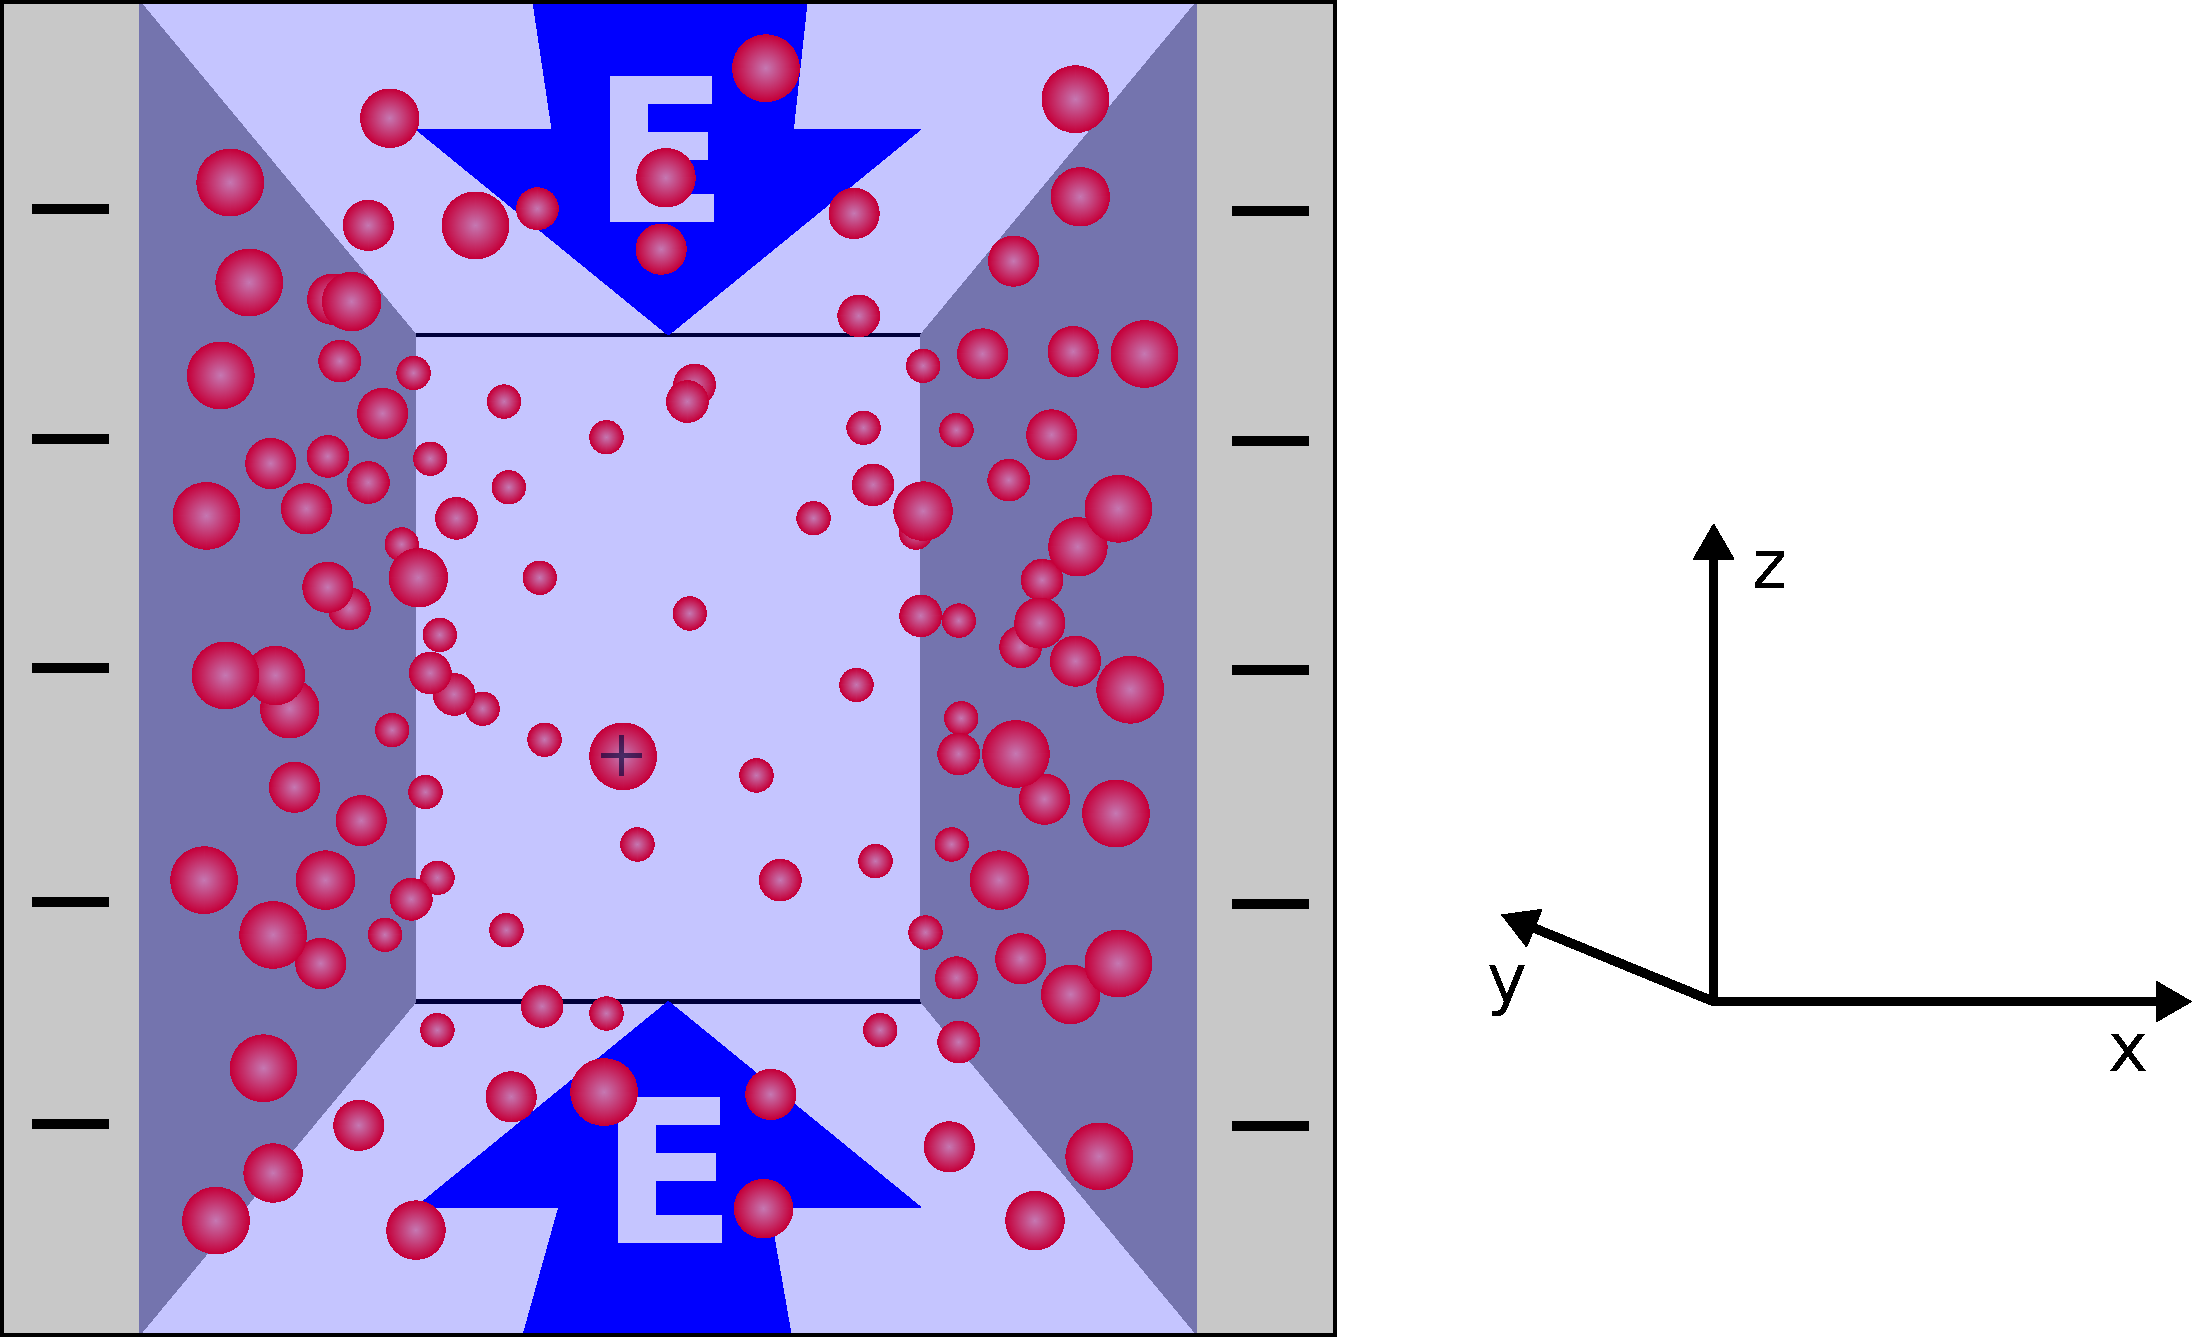
\includegraphics[width=0.5\columnwidth]{figures/schlitzpore_3d.pdf}
  \end{center}
  \caption{\label{fig:slit_pore}Slit pore system and coordinate system used for the analytical calculations.}
\end{figure}

Due to the net neutrality of the system and the
translational symmetry in directions parallel to the plates, the potential
outside the two plates must be constant. This means that using periodic or
non-periodic boundary conditions makes no difference. As the system is in equilibrium in the normal direction, the electrokinetic~\cref{eq:flux,eq:conti,eq:poisson} for this dimension reduce to the Poisson-Boltzmann equation for the electrostatic potential, which reads
\begin{align}
	\partial_x^2 \Phi(x) = -4 \pi \, \kT \, \lb \, ze \, c_0 \cdot \exp{\left(-\frac{ze\Phi(x)}{\kT}\right)} \; ,
\end{align}
where $x$ denotes the direction normal to the plates. The constant $c_0$ has to be chosen such that charge neutrality is fulfilled.
Multiplying by $2 \partial_x \Phi(x)$ and applying the
inverse chain rule further reduces the equation to first order. Subsequent
separation of variables yields the solution
\begin{align}
  \Phi(x) = -\frac{\kT}{ze} \cdot \log \left[ \frac{C^2}{8 \pi \, \kT \, \lb} \cdot \cos^{-2}\left( \frac{zeC}{2 \kT} \cdot x\right) \right], \quad \left| \frac{zeC}{2 \kT} \cdot x \right| < \frac \pi 2\; . \label{eq:validation_pb_counterions}
\end{align}
Refer to~\cite{rempfer10a} for details on this calculation.
Knowing that the counterion density $c$ resembles a Boltzmann distribution in the
potential $ze \Phi$ leads to the expression
\begin{align}
  c(x) = \frac{C^2}{8 \pi \, \kT \, \lb} \cdot \cos^{-2} \left( \frac{zeC}{2 \kT} \cdot x \right) \; . \label{eq:validation_pb_density}
\end{align}
The constant $C$ is determined by fixing the number of counterions or requiring
the E-field to vanish outside the volume contained by the plates. Both yields
\begin{align}
  C \cdot \tan \left( \frac{zed}{4 \kT} \cdot C \right) = -4 \pi \, \kT \, \lb \sigma \; ,
\end{align}
where $d$ denotes the distance between the plates and $\sigma$ their (constant) surface
charge density.

Applying an electrical field along one of the directions
parallel to the plates does not influence the charge distribution in the normal direction, which allows us to write down the hydrodynamic equations for the parallel direction. After eliminating all terms from the the Navier-Stokes Eqations~\eqref{eq:ns} which vanish due to symmetry, we are left with
\begin{align}
  \frac{\partial_x^2 v_y(x)}{\partial x^2} = -\frac{q E C^2}{8 \, \kT \, \lb \, \eta} \cdot \cos^{-2} \left( \frac{qC}{2 \kT} \cdot x \right) \; ,
\end{align}
which yields, by means of simple integration and the application of no-slip
boundary conditions
\begin{align}
  v_y(x) = \frac{E}{2 \pi \, \lb \, \eta \, ze} \cdot \log \left[ \frac{\cos \left( \frac{zeC}{2 \kT} \cdot x \right)}{\cos \left( \frac{zeC}{2 \kT} \cdot \frac d 2 \right)} \right] \; .
\end{align}
Here $x$ stands for the direction normal to the plates and $y$ for the direction of the
E-field and parallel to the plates.

With this tutorial comes a Python script \texttt{eof\_analytical.py}, which evaluates all these expressions on the same grid as is used in the simulation from section~\ref{sec:simulation}.

\pagebreak
